\documentclass{beamer}
\usetheme{Luebeck}
\usefonttheme{serif}
\usecolortheme{dove}
\useoutertheme{split}
%\useinnertheme{circles}
\usepackage[english]{babel}
\usepackage{graphicx}

\setbeamertemplate{footline}{}

\beamertemplatenavigationsymbolsempty

\usepackage[utf8]{inputenc}
\usepackage[T1]{fontenc}

\title{National Stereotypes in Whiskey Advertisement}
\institute{Institut für Anglistik\\Universität Leipzig}
\author{Hannes Eichblatt}
\date{12 July 2012}

\keywords{whiskey, whisky, stereotypes, advertisement, culture studies}
\subject{National Stereotypes in Whiskey Advertisement}

\begin{document}
\frame[plain]{\maketitle}

\section{Introduction}
\subsection{}

\begin{frame}
 \frametitle{Hypothesis}
 \begin{block}{I argue that}
  Advertisements use stereotypes as shortcuts to connect a product with positively connotated characteristics originally attributed to the country of production.
 \end{block}
\end{frame}

\begin{frame}
 \frametitle{Structure}
 \tableofcontents[]
\end{frame}

\section{Whiskey in and of itself}
\subsection{History}

\begin{frame}
 \frametitle{History}
\end{frame}

\subsection{Production}

\begin{frame}
 \frametitle{Production}
\end{frame}

\subsection{Etymology}

\begin{frame}
 \frametitle{Etymology}
 % Whisky, Whiskey?
\end{frame}
  
\section{Stereotypes}

\subsection{Definition}

\begin{frame}
 \frametitle{Defining Stereotypes}
  \begin{Definition}
    TODO Eine Definition
  \end{Definition}
\end{frame}

\subsection{Relevance}

\begin{frame}
 \frametitle{Relevance of stereotypes in cultural studies}
 \begin{quotation} %TODO
   All official institutions of language are repeating machines: school, sports, advertising, popular songs, news, all continually repeat the same structure, the same meaning, often the same words: the stereotype is a political fact, the major figure of ideology.\\
 \end{quotation}
 Roland Barthes "Modern," The Pleasure of the Text (1975)
\end{frame}

\subsection{Role in Advertisement}

\begin{frame}
 \frametitle{Stereotypes' role in advertisement}
\end{frame}

\section{Examples}
\subsection{Ireland}

\begin{frame}
 \frametitle{Ireland}
 \begin{itemize}
  % Jameson "The Lost Barrel" resilience, nature, dedication, merchant, shore
  \item <1-> Jameson \emph{Fire}
  \item <2-> England, simple people of Ireland
  % Jameson | "Hurricane":http://www.youtube.com/watch?v=yF2IaDQa2c8 | Ireland | easygoing, understatement, weather, community |
  \item<3-> Tullamore Dew \emph{Glasses up}
  \item<4-> pub, unity under whiskey and singing, resilience
  \item<5-> Tullamore Dew \emph{Pure as friendship}
  \item<6-> friendship, rough nature/weather, sea, shore, roughness, redheads
  \item<7-> The Knot \emph{A Binding Agreement}
  \item<8> Irish accent, directness, swearing, originality, maturity, purity of simple
\end{itemize}
\end{frame}

\subsection{Scotland}

\begin{frame}
 \frametitle{Scotland}
 \begin{itemize}
  \item<1-> William Lawson's \emph{Haka and Kilts}
  \item<2-> kilts, haka, rugby, understatement, manliness
  \item<3-> Bell's \emph{Great Catch}
  \item<4-> ingenuity, community, nature, fishing, rugby
  \item<5-> Red Bowler \emph{That's Scotland}
  \item<6> kilts, roughness and pride, history, bagpipes, nature
 \end{itemize}
\end{frame}

\subsection{USA}

\begin{frame}
 \frametitle{USA}
 \begin{itemize}
  \item<1-> Jack Daniel's \emph{American as}
  \item<2-> independence, freedom, quality, purity of simple, rock
  \item<3-> Jack Daniel's \emph{Number 7}
  \item<4-> railroads, gambling, women, tradition
  \item<5-> Jack Daniel's \emph{Tenessee Whiskey}
  \item<6-> countryside, farming, freedom, small towns/heartland, purity of simple
 \end{itemize}
\end{frame}

\subsection{Common Characteristics}

\begin{frame}
 \frametitle{Common characteristics of Whiskey advertisements of each country}
 \begin{itemize}
  \item
 \end{itemize}
\end{frame}

\begin{frame}
 \frametitle{Common characteristics of all Whiskey advertisements}
 \begin{itemize}
  \item
 \end{itemize}
\end{frame}

\section{Conclusion}

\begin{frame}
 \frametitle{Conclusion}
 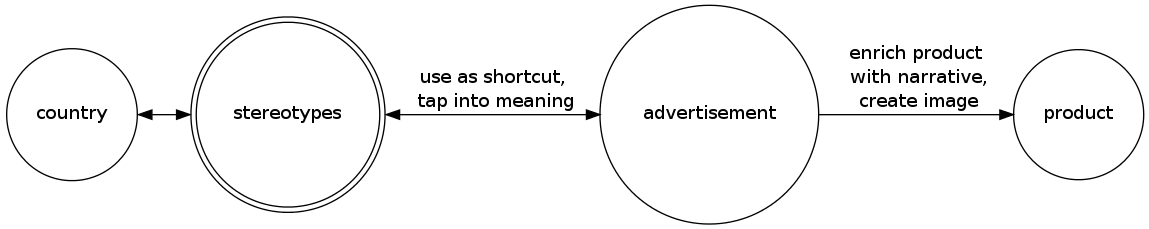
\includegraphics[scale=.25]{concepts.png}
\end{frame}

% \subsection{Fun fact (?)}
%| Canadian Club | "151 Countries, 1 Rye":http://www.youtube.com/watch?v=3H9wDdRk0vs | various | - |

\end{document}
